\documentclass[tikz,border=5pt]{standalone}
\usepackage{pgfplots}
\pgfplotsset{compat=1.18}
\definecolor{corba}{HTML}{365FB3}\definecolor{guia}{HTML}{7C3AED}\definecolor{punt}{HTML}{B91C1C}
\begin{document}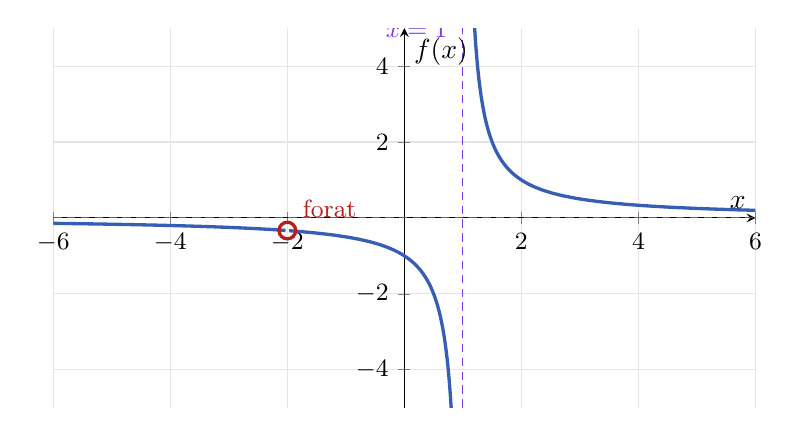
\begin{tikzpicture}
\begin{axis}[width=10.5cm,height=6.4cm,axis lines=middle,xmin=-6,xmax=6,ymin=-5,ymax=5,
 xlabel={$x$},ylabel={$f(x)$},grid=major,grid style={black!10},tick label style={font=\small},clip=true]
 \addplot[corba,very thick,domain=-6:-2.03,samples=160]{1/(x-1)};
 \addplot[corba,very thick,domain=-1.97:0.97,samples=160]{1/(x-1)};
 \addplot[corba,very thick,domain=1.03:6,samples=160]{1/(x-1)};
 \addplot[guia,densely dashed] coordinates {(1,-5) (1,5)};
 \addplot[guia,densely dashed,domain=-6:6]{0};
 \addplot[only marks,mark=o,mark size=3pt,very thick,punt,fill=white] coordinates {(-2,-0.3333)};
 \node[anchor=south east,font=\small,text=guia] at (axis cs:0.9,4.5) {$x=1$};
 \node[anchor=south west,font=\small,text=punt] at (axis cs:-1.9,-0.25) {forat};
\end{axis}\end{tikzpicture}\end{document}
